\DefineShortVerb{\!}
\chapter{Υλοποίηση}
\section{Υπάρχουσα ακολουθιακή υλοποίηση}
\subsection{Αρχική Κατάσταση Κώδικα}
\label{chapter:initial}
\noindent Ο κώδικας της υλοποίησης αναπτύχθηκε με βάση τον συνοδευτικό κώδικα της δημοσίευσης \cite{PlatisTheoharis03}. Η υλοποίηση αυτή παρέχει μια ολοκληρωμένη ακολουθιακή εκδοχή του αλγορίθμου που βασίζεται στην χρήση συντεταγμένων Plücker καθώς και άλλων αλγορίθμων τομής ευθείας-τετραέδρου οι οποίοι χρησιμοποιούνται για σύγκριση επιδόσεων. Επίσης παρέχει την υποδομή εισόδου και εξόδου για τα δεδομένα (ενότητα \ref{chapter:alginput}) και τα αποτελέσματα (ενότητα  \ref{chapter:algoutput}) του αλγορίθμου. Τέλος, παρέχει ένα σύστημα μέτρησης επιδόσεων το οποίο επιτρέπει την άμεση σύγκριση της ταχύτητας λειτουργίας των αλγορίθμων για τα ίδια δεδομένα εισόδου. Ο κώδικάς της είναι γραμμένος σε C++.

Ο κώδικας περιέχεται σε δύο καταλόγους, τους \verb!RayTetra! και \verb!Common!. Τα περιεχόμενά τους φαίνονται στους πίνακες \ref{Raytetra_contents} και \ref{Common_contents} αντίστοιχα. Ο \verb!RayΤetra! περιέχει το κύριο τμήμα του κώδικα της εφαρμογής, δηλαδή τον κώδικα των εκτελέσιμων και τις υλοποιήσεις των αλγορίθμων. O \verb!Common! περιέχει τους ορισμούς διάφορων κλάσεων που χρησιμοποιούνται συχνά στο υπόλοιπο της εφαρμογής. Για παράδειγμα, περιέχει τον ορισμό της κλάσης \verb!NpVector! η οποία περιγράφει όλα τα στοιχεία ενός τριδιάστατου διανύσματος. Επίσης στον κατάλογο \verb!Common! περιέχεται η υλοποίηση της κλάσης \begin{english}NpProgramTimer\end{english} μέσω της οποίας χρονομετρούνται οι αλγόριθμοι. 


\begin{table}[h!]
\centering
\caption{Περιεχόμενα του φακέλου \texttt{RayTetra}}
\label{Raytetra_contents}
\begin{tabular}{|l|l|l|}
\hline
Bench.cpp & BenchT.cpp & RayTetraT.cpp  \\ \hline
RandomRayTetra.cpp & RayTetra.cpp & RayTetraAlgorithms.cpp \\ \hline RayTetraAlgorithmsT.cpp & RayTetraHaines.cpp & RayTetraHainesT.cpp \\ \hline
RayTetraMoller.cpp & RayTetraSegura.cpp & RayTetraSeguraT.cpp \\ \hline
\end{tabular}\\[0.5cm]

\caption{Περιεχόμενα του φακέλου \texttt{Common}}
\label{Common_contents}
\begin{tabular}{|l|l|}
\hline
NpCArrayAdapter.hpp & NpPlane.hpp   \\ \hline
NpPluecker.hpp & NpProgramTimer.cpp \\ \hline
NpProgramTimer.hpp & NpUtil.hpp \\ \hline
NpVector.cpp & NpVector.hpp \\ \hline
\end{tabular}
\end{table}


Η υλοποίηση αυτή περιέχει τα εκτελέσιμα:

\begin{itemize}

\item \textbf{\verb!RayTetra!}: Το κυρίως εκτελέσιμο της υλοποίησης. Τρέχει έναν από τους αλγορίθμους τομής ευθείας-τετραέδρου, τον οποίο καθορίζει ο χρήστης, σε δεδομένα εισόδου τα οποία διαβάζονται από αρχείο κειμένου. Αποθηκεύει τα εξαγόμενα του αλγορίθμου και/ή τον χρόνο εκτέλεσής του σε αρχείο κειμένου. Επίσης παρέχει μια λειτουργία η οποία επιτρέπει την απεικόνιση του αποτελέσματος του αλγορίθμου για κάποιο δεδομένο ζεύγος ευθείας-τετραέδρου σε τριδιάστατα γραφικά. Η λειτουργία αυτή βασίζεται στην χρήση του OpenGL μέσω της βιβλιοθήκης glut.

\item \textbf{\verb!RandomRayTetra!}: Παράγει τυχαία δεδομένα εισόδου σε μορφή επεξεργάσιμη από το \verb!RayTetra!. Ο χρήστης καθορίζει τον αριθμό των τεμνόμενων και των μη τεμνόμενων ζευγών ευθείας-τετραέδρου που θα παραχθούν. Η ρύθμιση αυτή έχει ιδιαίτερη σημασία για την αξιολόγηση της απόδοσης των αλγόριθμων. Όπως επιδεικνύεται στο ~\cite{PlatisTheoharis03}, για να σχηματιστεί μια πλήρης εικόνα για την απόδοση ενός αλγορίθμου χρειάζεται η δοκιμή του σε διαφορετικές αναλογίες τεμνόμενων/μη τεμνόμενων ζευγών, καθώς η ροή ελέγχου της εκτέλεσής του διαφοροποιείται ανάλογα με την ύπαρξη ή μη ύπαρξη τομής.

\item \textbf{\verb!Bench!}: Μετρά την ταχύτητα εκτέλεσης των αλγορίθμων. Όλοι οι διαθέσιμοι αλγόριθμοι εκτελούνται σε κάποιο σύνολο δεδομένων εισόδου για ένα δοσμένο αριθμό επαναλήψεων. Οι χρόνοι εκτέλεσής τους εμφανίζονται στην οθόνη κατά την διάρκεια της χρονομέτρησης και καταγράφονται σε ένα αρχείο εξόδου με μορφή CSV (Comma Separated Values, τιμές διαχωρισμένες με κόμμα). Το αρχείο αυτό μπορεί να χρησιμοποιηθεί για την παραγωγή γραφικών παραστάσεων και στατιστικών στοιχείων.

\item \textbf{\verb!RayTetraT!, \verb!BenchT!}: Αντίστοιχα εκτελέσιμα με τα \verb!RayTetra! και \verb!Bench!. Αυτά περιλαμβάνουν την εκτέλεση τροποποιημένων εκδοχών των αλγορίθμων οι οποίες λαμβάνουν τα εσωτερικά γινόμενα συντεταγμένων \verb!Plücker! προϋπολογισμένα και χρονομετρούν μόνο τα κομμάτια της σύγκρισης των προσήμων και του καθορισμού των συντεταγμένων των σημείων τομής. Η λειτουργία αυτών των εκδοχών είναι εκτός των πλαισίων της εργασίας αυτής.

\end{itemize}


Στον κώδικα της δημοσίευσης η κάθε μορφή αλγορίθμου που χρησιμοποιείται περιέχεται σε μία συνάρτηση. Για να είναι δυνατόν να χρησιμοποιηθεί μια συνάρτηση-αλγόριθμος από το υπόλοιπο του κώδικα πρέπει να δίδεται προς αυτήν ένας δείκτης του τύπου \verb!(*RayTetraAlgo)! ο οποίος ορίζεται ως εξής: 

\begin{verbatim}
typedef bool (*RayTetraAlgo)(
    const NpVector &orig, 
    const NpVector &dir,
    const NpVector vert[],
    int &enterFace, int &leaveFace,
    NpVector &enterPoint, NpVector &leavePoint,
    double &uEnter1, double &uEnter2, 
    double &uLeave1, double &uLeave2,
    double &tEnter, double &tLeave);
\end{verbatim}
\verb!NpVector! ονομάζεται μια κλάση υλοποιημένη στο αρχείο \verb!Common!\textbackslash \verb!NpVector.h! της υλοποίησης η οποία αναπαριστά όλα τα στοιχεία που ορίζουν ένα τριδιάστατο διάνυσμα. Τα ορίσματα μιας συνάρτησης που αναπαριστά αλγόριθμο είναι τα εξής:\\


\noindent \verb!const NpVector &orig!: Το σημείο $P$ επί της ευθείας.\\
\noindent \verb!const NpVector dir!: Το διάνυσμα διεύθυνσης της ευθείας ($L$).\\
\noindent \verb!const NpVector vert[]!: Οι συντεταγμένες των ακμών του τετραέδρου $V_0$,$V_1$,$V_2$,$V_3$.\\
\noindent \verb!int enterFace!: Ο αριθμός (0-3) της έδρας του τετραέδρου στην οποία εισέρχεται η ευθεία, αν υπάρχει τομή.\\
\noindent \verb!int leaveFace!: Ο αριθμός (0-3) της έδρας από την οποία εξέρχεται η ευθεία.\\
\noindent \verb!NpVector enterPoint!: Οι καρτεσιανές συντεταγμένες του σημείου εισόδου.\\
\noindent \verb!NpVector leavePoint!: Οι καρτεσιανές συντεταγμένες του σημείου εξόδου.\\
\noindent \verb!double uEnter1, double uEnter2!: Οι βαρυκεντρικές συντεταγμένες του σημείου εισόδου $u^{enter}_1$ και $u^{enter}_2$. \\
\noindent \verb!double uLeave1, double uLeave2!: Οι βαρυκεντρικές συντεταγμένες του σημείου εξόδου $u^{leave}_1$ και $u^{leave}_2$.\\
\noindent \verb!double tEnter, double tLeave!:  Οι παραμετρικές αποστάσεις των σημείων εισόδου και εξόδου, $t_{enter}$ και $t_{leave}$,  από το σημείο $P$ .\\

Οι αλγόριθμοι ενσωματώνονται στα εκτελέσιμα μέσω του αρχείου \begin{english}header \verb!RayTetraAlgorithms.hpp!\end{english}. Το αρχείο αυτό περιέχει όλα τα πρωτότυπα των συναρτήσεων-αλγορίθμων. Ο πλήρεις ορισμοί των συναρτήσεων βρίσκονται στα αρχεία πηγαίου κώδικα \begin{english}\verb!RayTetraHaines.cpp!\end{english}, \begin{english}\verb!RayTetraMoller.cpp!\end{english} καί \begin{english}\verb!RayTetraSegura.cpp!\end{english}.

Ο κώδικας στην αρχική του μορφή περιλαμβάνει τον αλγόριθμο τομής με συντεταγμένες Plücker στο αρχείο \verb!RayTetraSegura.cpp!. Περιέχει και τις τρεις μορφές του αλγορίθμου που παρουσιάστηκαν στο κεφάλαιο \ref{chapter:algs}. Στο κείμενο του κώδικα οι μορφές αυτές ονομάζονται ως εξής:\\

\noindent \verb!RayTetraSegura0! = Βασικός Αλγόριθμος (μορφή 0).\\
\verb!RayTetraSegura1! = Βασικός Αλγόριθμος με βελτιστοποιήσεις ελέγχου και επανάληψη χρήσης υπολογισμένων ποσοτήτων (μορφή 1).\\
\verb!RayTetraSegura2! = Βασικός Αλγόριθμος με βελτιστοποιήσεις ελέγχου, επανάληψη χρήσης υπολογισμένων ποσοτήτων και γεωμετρική βελτιστοποίηση (μορφή 2).\\
Τα υπόλοιπα αρχεία, RayTetraHaines.cpp και RayTetraMoller.cpp περιέχουν άλλες παραλλαγές του αλγορίθμου που είχαν χρησιμοποιηθεί στα πλαίσια της δημοσίευσης και δεν αφορούν την παρούσα εργασία.

Η προϋπάρχουσα αυτή υλοποίηση έχει αναπτυχθεί με σκοπό την εκτέλεση σε λειτουργικό σύστημα Linux. Η μεταγλώττιση του κώδικα και η δημιουργία των εκτελέσιμων αρχείων γίνεται με την χρήση makefile.

\subsection{Δομή αρχείων εισόδου-εξόδου}
\noindent Τα αρχεία εισόδου και εξόδου είναι απλά αρχεία κειμένου με την εξής δομή:

\paragraph{Αρχεία εισόδου:} Η πρώτη γραμμή κάθε αρχείου εισόδου περιέχει τον αριθμό των ζευγών ευθείας-τετραέδρου που περιγράφονται στο αρχείο. Κάθε γραμμή που ακολουθεί περιέχει τις συντεταγμένες που προσδιορίζουν ένα ζεύγος. Τα στοιχεία αυτά είναι αριθμοί κινητής υποδιαστολής και διαχωρίζονται με κενά. Οι συνιστώσες σε κάθε άξονα (x,y,z) των συντεταγμένων κάθε σημείου διαχωρίζονται επίσης με κενά. Τα στοιχεία αναγράφονται με την σειρά:
\begin{enumerate*}
\item Συντεταγμένες κορυφής $V_0$ 
\item Συντεταγμένες κορυφής $V_1$
\item Συντεταγμένες κορυφής $V_2$
\item Συντεταγμένες κορυφής $V_3$ 
\item Συντεταγμένες σημείου P
\item Συντεταγμένες διανύσματος L
\end{enumerate*}

\paragraph{Αρχεία εξόδου:} Κάθε γραμμή περιέχει τα εξαγόμενα του αλγορίθμου για ένα ζεύγος ευθείας-τετραέδρου. Το πρώτο εξαγόμενο είναι μία λογική (boolean) μεταβλητή η οποία δηλώνει αν υπάρχει τομή ή όχι. Αν υπάρχει τότε ακολουθούν τα υπόλοιπα στοιχεία που την προσδιορίζουν. Αν όχι η γραμμή τερματίζεται. Τα στοιχεία της τομής αναγράφονται ως εξής: 

\begin{enumerate*}
\item Λογική τιμή ύπαρξης τομής
\item Αριθμός έδρας εισόδου $F_{enter}$
\item Αριθμός έδρας εξόδου $F_{leave}$
\item Καρτεσιανές συντεταγμένες σημείου εισόδου $P_{enter}$
\item Καρτεσιανές συντεταγμένες σημείου εξόδου $P_{leave}$
\item Βαρυκεντρικη συνιστώσα 1 σημείου εισόδου $u^{enter}_1$
\item Βαρυκεντρικη συνιστώσα 2 σημείου εισόδου $u^{enter}_2$
\item Βαρυκεντρικη συνιστώσα 1 σημείου εξόδου $u^{leave}_1$
\item Βαρυκεντρικη συνιστώσα 2 σημείου εξόδου $u^{leave}_2$
\item Παραμετρική απόσταση $t_{enter}$
\item Παραμετρική απόσταση $t_{leave}$
\end{enumerate*}

\section{Προσθήκες στην ακολουθιακή υλοποίηση}

\noindent Τα νέα τμήματα κώδικα που αναπτύχθηκαν στα πλαίσια αυτής της εργασίας χρησιμοποιούν τις προϋπάρχουσες υποδομές εισόδου-εξόδου και μέτρησης επιδόσεων καθώς και τις διεπαφές χρήστη της υπάρχουσας υλοποίησης. Αυτό γίνεται για τους εξής λόγους:

\begin{itemize}
\item Δυνατότητα άμεσης σύγκρισης και επαλήθευσης των αποτελεσμάτων των νέων αλγορίθμων. Τα δεδομένα εισόδου και τα εξαγόμενα κάθε αλγορίθμου γράφονται σε αρχεία κειμένου με το ίδιο ακριβώς συντακτικό, ανεξάρτητα από την αναπαράσταση που χρησιμοποιείται εσωτερικά στον καθένα. Αυτό επιτρέπει την άμεση και αυτοματοποιημένη σύγκριση μεταξύ των στοιχείων αυτών όπως παράγονται από ή εισάγονται σε κάθε αλγόριθμο. Με την μέθοδο αυτή η επαλήθευση των αποτελεσμάτων των νέων αλγορίθμων μπορεί να γίνει εύκολα μέσω της σύγκρισης τους με αυτά των υπαρχόντων. Για τον σκοπό αυτό έχει αναπτυχθεί το \verb!result_compare!, ένα bash script το οποίο βασίζεται στην εφαρμογή \verb!diff! του περιβάλλοντος GNU/Linux. Η χρήση του θα περιγραφεί σε μεγαλύτερο βαθμό στην συνέχεια του κειμένου. 
\item Δυνατότητα χρήσης του εκτελέσιμου \verb!RandomRayTetra! για την παραγωγή αρχείων εισόδου με τυχαία στοιχεία. Η χρήση της υπάρχουσας υποδομής εισόδου-εξόδου επιτρέπει στους νέους αλγόριθμους να χρησιμοποιούν ως είσοδο τα αρχεία που παράγονται από το \verb!RandomRayTetra!. Έτσι διευκολύνθηκε σημαντικά η ανάπτυξη και ο έλεγχος των νέων αλγορίθμων. Η παραγωγή στοιχείων εισόδου με ικανό μέγεθος και εύρος τιμών ώστε να χρησιμοποιηθούν για τον έλεγχο της λειτουργίας των αλγορίθμων θα ήταν εξαιρετικά δύσκολο να γίνει χωρίς την χρήση του.
\item Δυνατότητα άμεσης σύγκρισης των επιδόσεων των νέων αλγοριθμικών μορφών με τις υπάρχουσες μέσω του εκτελέσιμου \verb!Bench!.
\item Παροχή μίας ενιαίας και συνεκτικής διεπαφής χρήστη για όλες τις διαθέσιμες υλοποιήσεις των αλγορίθμων τομής ευθείας-τετραέδρου, συμπεριλαμβανομένης και της υλοποίησης OpenCL η οποία θα παρουσιαστεί στην συνέχεια.
\end{itemize}


\subsection{Ακολουθιακός αλγόριθμος μεικτού γινόμενου}

\noindent Ο πρώτος στόχος του πρακτικού τμήματος της εργασίας ήταν η δημιουργία και ενσωμάτωση μιας ακολουθιακής εκδοχής του αλγόριθμου τομής ευθείας-τετραέδρου με μεικτό γινόμενο. Οι μορφές του αλγορίθμου αυτού ονομάστηκαν RayTetraSTP 0,1 και 2 κατ' αντιστοιχία με τις ήδη υλοποιημένες. Ο ορισμός τους βρίσκεται στο αρχείο RayTetra\textbackslash RayTetraSTP.cpp που περιέχεται στα παραδοτέα της εργασίας.

Η ανάπτυξη του αλγόριθμου αυτού βασίστηκε στην μετατροπή του αλγορίθμου τομής με συντεταγμένες Plücker. Η ουσιαστική διαφορά των δύο αλγορίθμων βρίσκεται στον υπολογισμό διαφορετικών ποσοτήτων: Αντιμετατεθημένων εσωτερικών γινομένων συντεταγμένων Plücker ή μεικτών γινομένων. Καθώς οι δύο αλγόριθμοι εκτελούν τους ίδιους ακριβώς υπολογισμούς με τις δύο αυτές ποσότητες, η αντικατάσταση των τμημάτων κώδικα που τις υπολογίζουν μπορούν να μετατρέψει τον ένα στον άλλο. 

Μία σημαντική διαφορά είναι ότι στον αλγόριθμο με μεικτό γινόμενο απαιτείται η προσθήκη κώδικα για την μετατροπή των συντεταγμένων των κορυφών του τετραέδου με αφαίρεση του διανύσματος $P$. Όπως αναφέρθηκε στην παράγραφο \ref{chapter:stpalg}, για να μπορούν να χρησιμοποιηθούν οι συντεταγμένες των κορυφών του τετραέδρου από τον αλγόριθμο πρέπει να αφαιρεθούν από αυτές οι συντεταγμένες του σημείου $P$. Στον κώδικα αυτό μεταφράζεται σε αφαίρεση του διανύσματος \verb!orig! από όλα τα διανύσματα στον πίνακα \verb!vert[]!. 

Η κυριότερη διαφοροποίηση των δύο αλγορίθμων, η οποία αποτελεί και τον λόγο χρήσης του αλγορίθμου με μεικτό γινόμενο ως προτιμότερο του αλγορίθμου συντεταγμένων Plücker, είναι ο μικρότερος αριθμός διανυσματικών πράξεων οι οποίες είναι απαραίτητο να εκτελεστούν. Η διαφορά είναι έκδηλη αν εξεταστούν οι χείριστες περιπτώσεις εκτέλεσης των δύο αλγορίθμων, δηλαδή αυτές στις οποίες πρέπει να εξεταστούν όλες οι έδρες του τετραέδρου για να προσδιοριστεί η τομή. Στην περίπτωση αυτή ο αλγόριθμος Plücker πρέπει να υπολογίσει 7 συντεταγμένες Plücker οι οποίες αναλογούν στην ευθεία και στις 6 ακμές του τετραέδρου. Ο κάθε υπολογισμός απαιτεί μια πράξη εξωτερικού γινομένου [σχέση \eqref{eq:plucker}]. Στη συνέχεια πρέπει να παραχθούν 6 γινόμενα συντεταγμένων Plücker. Κάθε ένα από αυτά είναι το γινόμενο των συντεταγμένων της ευθείας με αυτές κάποιας ακμής του τετραέδρου. Το κάθε τέτοιο γινόμενο απαιτεί 2 πράξεις εσωτερικού γινομένου [σχέση \eqref{eq:permuted}]. Συνολικά, ο αλγόριθμος αυτός στην χείριστη περίπτωση απαιτεί τον 
υπολογισμό 7 εξωτερικών και 12 εσωτερικών γινομένων. Στην ίδια περίπτωση, ο αλγόριθμος μεικτού γινομένου απαιτεί σημαντικά λιγότερες πράξεις. Κάθε ακμή του τετραέδρου απαιτεί τον υπολογισμό ενός μεικτού γινομένου. Το κάθε μεικτό γινόμενο απαιτεί 1 εξωτερικό και ένα εσωτερικό γινόμενο. Χρησιμοποιώντας τις ιδιότητες του μεικτού γινομένου [σχέσεις \eqref{eq:circular} και \eqref{eq:noncircular}] είναι εφικτή η μείωση του αριθμού των εξωτερικών γινομένων που πρέπει να υπολογιστούν σε 3. Συνολικά, ο αλγόριθμος αυτός στην χείριστη περίπτωση απαιτεί 3 εξωτερικά και 6 εσωτερικά γινόμενα για την εξέταση όλων των ακμών του τετραέδρου, πρακτικά τα μισά από αυτά του αλγορίθμου  Plücker. Πρέπει να σημειωθεί ότι ο ορισμός της χείριστης περίπτωσης που χρησιμοποιείται στο παραπάνω κείμενο αφορά την μη βελτιστοποιημένη μορφή 0 των αλγορίθμων.

Μετά το πέρας της υλοποίησης των τριών μορφών του αλγορίθμου η ενσωμάτωσή τους στα εκτελέσιμα του υπάρχοντος κώδικα ήταν σχετικά απλή. Τα πρωτότυπα των τριών συναρτήσεων προστέθηκαν στο αρχείο πηγαίου κώδικα \begin{english}\verb!RayTetraAlgorithms.cpp!\end{english}. Επίσης, τροποποιήθηκε ο κώδικας των εκτελέσιμων \verb!RayTetra! και \verb!Bench! ώστε να προστεθούν σε αυτά νέες επιλογές χρήστη και κλήσεις συναρτήσεων  για την επιλογή των νέων αλγορίθμων. Στο \verb!Bench! προστέθηκε μια επιπλέον εγγραφή εξόδου για τους νέους αλγορίθμους έτσι ώστε να είναι δυνατή η σύγκριση των επιδόσεών τους με τους προϋπάρχοντες.
  

\section{Υλοποίηση OpenCL}

\subsection{Δομή}

\noindent Το κύριο ζητούμενο της εργασίας αυτής ήταν η δημιουργία μίας υλοποίησης των αλγορίθμων που παρουσιάστηκαν στο κεφάλαιο \ref{chapter:algs} σε μορφή προορισμένη προς επεξεργασία σε GPU. Για τον σκοπό αυτό, όπως αναφέραμε στην ενότητα \ref{chapter:apis}, επιλέχθηκε το πρότυπο OpenCL. 

Σύμφωνα με το μοντέλο επεξεργασίας του OpenCL \cite{OpenCLSpec} κάθε πρόγραμμα που αναπτύσσεται σε αυτό το πρότυπο αποτελείται από δύο τμήματα. Το πρώτο είναι το \textit{πρόγραμμα host} το οποίο είναι ένα ακολουθιακό πρόγραμμα που εκτελείται από την CPU του συστήματος που περιέχει την  συσκευή-στόχο η οποία θα αναλάβει τον υπολογισμό (στην περίπτωση αυτή η GPU). Το πρόγραμμα host αναλαμβάνει την αναγνώριση συσκευών συμβατών με το OpenCL, τον προγραμματισμό τους, τον έλεγχο της λειτουργίας τους και την μεταφορά δεδομένων προς και από αυτές. Το δεύτερο τμήμα ενός προγράμματος OpenCL είναι \textit{οι πυρήνες υπολογισμού} (computation kernels). Όπως αναφέραμε στην ενότητα \ref{chapter:openclraytetra}, ο κάθε πυρήνας είναι μια συνάρτηση η οποία εκτελείται στην GPU και αναλαμβάνει κάποιο υπολογιστικά εντατικό τμήμα της εφαρμογής. Ο κάθε πυρήνας εκτελείται παράλληλα για ένα μεγάλο πλήθος των δεδομένων εισόδου.  

Ακολουθώντας το μοντέλο αυτό, η υλοποίηση αυτή αποτελείται από δύο βασικά τμήματα. Το πρώτο είναι μια βιβλιοθήκη συναρτήσεων η οποία ονομάστηκε \verb!gpuHandler!. H βιβλιοθήκη αυτή παρέχει στα εκτελέσιμα \verb!RayTetra! και \verb!Bench! δυνατότητες χρήσης της GPU για την εκτέλεση υπολογισμών. Η λειτουργίες της \verb!gpuHandler! αποτελούν συνολικά το host πρόγραμμα της υλοποίησης. Ο πηγαίος κώδικάς της βρίσκεται στα αρχεία \begin{english}\verb!gpuHandler.hpp!\end{english} και \begin{english}\verb!gpuHandler.cpp!\end{english}. Το δεύτερο τμήμα είναι οι πυρήνες επεξεργασίας. Στην εφαρμογή της εργασίας ο κάθε πυρήνας περιέχει μια πλήρη υλοποίηση ενός αλγόριθμου τομής ευθείας-τετραέδρου. Η υλοποίηση αυτή έχει επικεντρωθεί στον αλγόριθμο μεικτού γινομένου λόγω της υψηλότερης απόδοσής του. Έχουν υλοποιηθεί οι τρεις μορφές του αλγορίθμου μεικτού γινομένου όπως παρουσιάστηκαν στο κεφάλαιο \ref{chapter:algs}, καθώς και η μορφή 0 του αλγορίθμου συντεταγμένων Plücker. Ο κώδικας κάθε πυρήνα περιέχεται σε ένα ανεξάρτητο 
αρχείο με την κατάληξη .cl. Έτσι, τα αρχεία που περιέχουν τον πηγαίο κώδικα των πυρήνων ονομάζονται ως εξής: \begin{center}\verb!RayTetra[όνομα αλγορίθμου][Αριθμός Μορφής].cl!.\end{center}
 
Η ανάπτυξη της υλοποίησης αυτής έγινε σε περιβάλλον Linux. Έχουν παραχθεί εκτελέσιμα αρχεία για περιβάλλον Linux και Windows. Η προσαρμογή της εφαρμογής στην εκτέλεση σε περιβάλλον Windows έγινε με χρήση του περιβάλλοντος ανάπτυξης \begin{english}Visual Studio\end{english} της Μicrosoft. Και στα δύο λειτουργικά συστήματα χρησιμοποιήθηκαν οι διεπαφές προγραμματισμού \begin{english}AMD APP (Accelerated Parallel Processing) SDK\end{english} (\url{http://developer.amd.com/sdks/AMDAPPSDK/Pages/default.aspx}), η οποία είναι μια σειρά εργαλείων ανάπτυξης λογισμικού της εταιρίας AMD για την ανάπτυξη εφαρμογών OpenCL με στόχο τις GPU και παρεμφερείς συσκευές της AMD, και CUDA Toolkit (\url{http://developer.nvidia.com/cuda-toolkit}), η οποία είναι το αντίστοιχο περιβάλλον για τις συσκευές της Nvidia. Ο κώδικας της βιβλιοθήκης \begin{english}gpuHandler\end{english} έχει γραφτεί σε C++ χρησιμοποιώντας τα C bindings του ΟpenCL. Οι πυρήνες έχουν γραφτεί σε OpenCL C. 

Όπως αναφέρθηκε στο κεφάλαιο \ref{chapter:apis}, ο κυριότερος λόγος επιλογής του προτύπου OpenCL για την υλοποίηση της εργασίας είναι η ευρεία υποστήριξή του σε συσκευές πολλών διαφορετικών τύπων που προέρχονται από  διαφορετικούς κατασκευαστές. Στα πλαίσια της ανάπτυξής του ο κώδικας της εργασίας έχει δοκιμαστεί σε GPU της AMD καί της Nvidia καθώς και σε πολυπύρηνο CPU της AMD. Με τις κατάλληλες προβλέψεις στον κώδικα η ίδια εφαρμογή λειτουργεί και στις τρεις αυτές συσκευές χωρίς τροποποίηση, παράγοντας πρακτικά πανομοιότυπα εξαγόμενα με ικανοποιητικό επίπεδο επιδόσεων. Η μοναδική διαφοροποίηση μεταξύ των εξαγομένων που προέρχονται από τις συσκευές αυτές προέρχεται από την διαφορετική ακρίβεια που χρησιμοποιούν στην αναπαράσταση αριθμών κινητής υποδιαστολής. Η διαφορά αυτή έχει ως αποτέλεσμα την εμφάνιση μικρών αριθμητικών διαφορών η οποίες προέρχονται από την στρογγυλοποίηση της αναπαράστασης σε διαφορετικά δεκαδικά ψηφία.

\subsection{Θέματα σχεδιασμού}
\label{chapter:design}

\noindent Για να γίνουν κατανοητές οι σχεδιαστικές επιλογές που ακολουθήθηκαν στην υλοποίηση αυτή είναι απαραίτητο να γίνει μια αναφορά σε τρεις σημαντικές έννοιες οι οποίες έχουν βασική σημασία στην ανάπτυξη λογισμικού με το OpenCL και την διαφοροποιούν σημαντικά από την ανάπτυξη ακολουθιακών προγραμμάτων. Οι έννοιες αυτές είναι ο ορισμός του χώρου προβλήματος, το μοντέλο μνήμης του OpenCL και η μέθοδος μεταγλώττισης πυρήνων.

\subsubsection*{Ορισμός Χώρου Προβλήματος}

\noindent Το πρότυπο OpenCL εκμεταλλεύεται την παραλληλία του υλικού των GPU χρησιμοποιώντας πρακτικές εμπνευσμένες από την παραλληλία SIMD. Αυτό επιτυγχάνεται με τον κατακερματισμό της ζητούμενης επεξεργασίας σε πολλά ανεξάρτητα υπολογιστικά στοιχεία καθένα από τα οποία εκτελεί την ίδια  συνάρτηση-πυρήνα. Το κάθε ένα από αυτά τα στοιχεία έχει πρόσβαση σε ένα διαφορετικό τμήμα των δεδομένων εισόδου του προγράμματος και παράγει το αντίστοιχο τμήμα των δεδομένων εξόδου. Ο τρόπος αντιστοίχισης των τμημάτων της επεξεργασίας στα επιμέρους υπολογιστικά στοιχεία ονομάζεται \textit{ορισμός χώρου προβλήματος}.

Ο χώρος προβλήματος ορίζεται ως ένας ν-διάστατος χώρος δεικτών. Κάθε υπολογιστικό στοιχείο του χώρου αυτού ονομάζεται \textit{αντικείμενο εργασίας} (work item). Το κάθε στοιχείο εργασίας είναι στην ουσία μία πλήρης εκτέλεση του κώδικα ενός πυρήνα. Καταχρηστικά μπορεί να θεωρηθεί ότι η έννοια του στοιχείου επεξεργασίας στο OpenCL αντιστοιχεί με αυτή του νήματος (thread) επεξεργασίας στα περισσότερα συστήματα παράλληλης επεξεργασίας. Σύμφωνα με την θέση του στοιχείου εργασίας στο χώρο προβλήματος του ανατίθεται ένας αριθμός με βάση τον οποίο υπολογίζεται η θέση μνήμης των δεδομένων εισόδου και εξόδου που του αναλογούν. 
 
Στις υλοποιήσεις του OpenCL που είχαν αναπτυχθεί μέχρι την συγγραφή του κειμένου αυτού ο χώρος προβλήματος μπορεί να αποτελείται από μία, δύο ή τρεις διαστάσεις. Μια επεξεργασία η οποία εφαρμόζεται πάνω σε γραμμικές δομές δεδομένων, π.χ. λίστες, αντιστοιχεί σε μονοδιάστατο χώρο προβλήματος. Αντίστοιχα, η επεξεργασία μιας διδιάστατης εικόνας (για παράδειγμα, ένα φίλτρο εικόνας όπως αυτά που χρησιμοποιούνται στα προγράμματα επεξεργασίας γραφικών) αντιστοιχεί σε διδιάστατο χώρο προβλήματος. Σε τριδιάστατο χώρο προβλήματος μπορεί να αντιστοιχηθεί, μεταξύ άλλων, ένας μετασχηματισμός ενός γεωμετρικού όγκου, ένα κοινό πρόβλημα στα τριδιάστατα γραφικά. Στην γενική περίπτωση ο αριθμός των διαστάσεων του χώρου προβλήματος καθορίζεται από την μορφή των δεδομένων εισόδου. Ο αριθμός των αντικειμένων εργασίας που δημιουργούνται σε μία εκτέλεση ενός πυρήνα ονομάζεται \textit{ολικό μέγεθος} (global size) του χώρου προβλήματος. Στην υλοποίηση της εργασίας χρησιμοποιείται μονοδιάστατος χώρος προβλήματος. καθώς τα δεδομένα 
εισόδου είναι μονοδιάστατοι πίνακες αριθμών κινητής υποδιαστολής.

Στην μεγάλη πλειοψηφία των παράλληλων εφαρμογών το αποτέλεσμα της επεξεργασίας του κάθε αντικειμένου εργασίας δεν εξαρτάται μόνο από τα δεδομένα εισόδου του αλλά και από την κατάσταση κάποιων από τα υπόλοιπα αντικείμενα εργασίας. Αυτό σημαίνει ότι υπάρχουν εξαρτήσεις δεδομένων μεταξύ των εντολών που εκτελούνται σε διαφορετικά αντικείμενα εργασίας. Για την ικανοποίηση των εξαρτήσεων αυτών απαιτείται να υπάρχει ανταλλαγή δεδομένων μεταξύ των αντικειμένων εργασίας και μηχανισμοί συγχρονισμού για την διασφάλιση της εγκυρότητας των στοιχείων που ανταλλάσσονται. Το OpenCL αντιμετωπίζει αυτό το πρόβλημα με την ομαδοποίηση των αντικειμένων εργασίας σε \textit{ομάδες εργασίας} (workgroups). Τα αντικείμενα εργασίας που ανήκουν στην ίδια ομάδα έχουν κοινή πρόσβαση σε μια περιοχή μνήμης η οποία ονομάζεται \textit{τοπική μνήμη} (local memory), μέσω της οποίας μπορούν να ανταλλάσσουν δεδομένα. Επίσης εντός της ίδιας ομάδας εργασίας παρέχεται η δυνατότητα συγχρονισμού μεταξύ των αντικειμένων εργασίας με την χρήση \textit{
εντολών-φραγμάτων} (barrier). Ο αριθμός των αντικειμένων εργασίας που περιέχονται σε κάθε ομάδα εργασίας ονομάζεται \textit{τοπικό μέγεθος} (local size) του χώρου προβλήματος. Το τοπικό μέγεθος πρέπει να διαιρεί ακέραια το ολικό.

Ο ορισμός του τοπικού μεγέθους σε κάποια εφαρμογή OpenCL έχει καθοριστική σημασία για την απόδοση της εφαρμογής, άσχετα αν η εφαρμογή αυτή απαιτεί μεταφορά δεδομένων ή συγχρονισμό μεταξύ αντικειμένων εργασίας. Το γεγονός αυτό προκύπτει από τον αρχιτεκτονικό σχεδιασμό των σύγχρονων GPU. Κάθε GPU αποτελείται από έναν αριθμό ανεξάρτητων υπολογιστικών μονάδων. Κάθε μία από αυτές τις μονάδες περιέχει υπολογιστικά στοιχεία ικανά να εκτελέσουν μερικές δεκάδες ή εκατοντάδες αντικείμενα εργασίας παράλληλα. Για να είναι δυνατή η επικοινωνία μεταξύ κάποιων αντικειμένων εργασίας μέσω της τοπικής μνήμης πρέπει αυτά να εκτελούνται στην ίδια υπολογιστική μονάδα, καθώς η τοπική μνήμη κάθε τέτοιας μονάδας είναι ανεξάρτητη. Σε αυτές τις συνθήκες είναι αδύνατον ένα αντικείμενο εργασίας να εκτελείται αν δεν εκτελούνται παράλληλα και όλα τα υπόλοιπα που ανήκουν στην ομάδα εργασίας του. Γι' αυτό, η υλοποίηση του OpenCL αναθέτει την εκτέλεση των αντικειμένων εργασίας στις υπολογιστικές ομάδες χρησιμοποιώντας ως ελάχιστη μονάδα την 
ομάδα εργασίας. Αυτό σημαίνει ότι μια υπολογιστική μονάδα ανά πάσα στιγμή μπορεί να εκτελεί μία ή περισσότερες ολόκληρες μονάδες εργασίας αλλά όχι υποσύνολα κάποιας ομάδας.  Παράλληλα, ο μέγιστος αριθμός ομάδων επεξεργασίας που μπορούν να εκτελούνται ανά πάσα στιγμή σε κάθε υπολογιστική μονάδα είναι μικρός. Οι περιορισμοί αυτοί συνολικά σημαίνουν ότι η επιλογή πολύ μικρού τοπικού μεγέθους περιορίζει τον συνολικό αριθμό των αντικειμένων εργασίας που μπορούν να εκτελεστούν παράλληλα στην GPU. Έτσι, είναι πιθανόν ένα τμήμα του υπολογιστικού υλικού να παραμείνει αδρανές, μειώνοντας δραστικά τις επιδόσεις.

Για να αποφευχθεί το πρόβλημα αυτό οι κατασκευαστές GPU συνιστούν την ανάθεση συγκεκριμένων τοπικών μεγεθών. Οι συνιστώμενοι αριθμοί είναι το 64 στις GPU της AMD και το 32 στις GPU της Nvidia καθώς και κάποια ακέραια πολλαπλάσιά τους. Στην εκτέλεση κώδικα OpenCL σε CPU και άλλες συσκευές διαφορετικής αρχιτεκτονικής το τοπικό μέγεθος αγνοείται. 

Στην εφαρμογή της εργασίας το ολικό και τοπικό μέγεθος υπολογίζονται ως εξής:

\begin{enumerate}
\item Αρχικά, προσδιορίζεται το είδος και ο κατασκευαστής της συσκευής όπου θα εκτελεστεί. Το API του OpenCL περιέχει κλήσεις οι οποίες μπορούν να ανιχνεύσουν τις συμβατές με OpenCL συσκευές που υπάρχουν στο σύστημα και να εξετάσουν τα διάφορα στοιχεία τους (όνομα, κατασκευαστής, ποσότητα μνήμης, δυνατότητες κ.α.). Σε περίπτωση που υπάρχουν πάνω από μία συμβατές συσκευές ο χρήστης έχει την δυνατότητα να επιλέξει μεταξύ τους. 
\item Ανάλογα με την επιλεγμένη συσκευή:
	\begin{itemize}
	\item Αν πρόκειται για GPU της AMD, το τοπικό μέγεθος παίρνει την τιμή 	64. Ο αριθμός αυτός βρέθηκε να αποδίδει τα καλύτερα αποτελέσματα από 		άποψη επιδόσεων στην συγκεκριμένη εφαρμογή.
	\item Αν πρόκειται για GPU της Nvidia, το τοπικό μέγεθος παίρνει την 		τιμή του μεγαλύτερου πολλαπλάσιου του 32 που επιτρέπεται από την 			υλοποίηση του OpenCL για τον συγκεκριμένο πυρήνα.
	\item Αν πρόκειται για οποιαδήποτε άλλη συσκευή το τοπικό μέγεθος 			παίρνει την τιμή 1. Η τιμή αυτή αγνοείται κατά την εκτέλεση του κώδικα 	αλλά είναι απαραίτητη για λόγους που θα διευκρινιστούν στο επόμενο βήμα.
  \end{itemize} 
\item Το ολικό μέγεθος αναπροσαρμόζεται ανάλογα με το τοπικό μέγεθος. Το ολικό μέγεθος αρχικά είναι ίσο με τον αριθμό ζευγών ευθείας-τετραέδρου που έχουν διαβαστεί απο το αρχείο εισόδου. Ο αριθμός αυτός συμπληρώνεται με εικονικά ζεύγη έτσι ώστε να φτάσει το επόμενο ακέραιο πολλαπλάσιο του τοπικού. Όλα τα στοιχεία των εικονικών ζευγών έχουν την τιμή 0 και τα αποτελέσματά της επεξεργασίας τους δεν επιστρέφονται από την GPU στο host πρόγραμμα. Επειδή η ανάθεση των αντικειμένων εργασίας στις υπολογιστικές μονάδες γίνεται με ελάχιστη μονάδα την ομάδα εργασίας η προσθήκη των εικονικών ζευγών δεν επηρεάζει την απόδοση του προγράμματος.
\end{enumerate}

\subsubsection*{Tο μοντέλο μνήμης του OpenCL}

\noindent Το μοντέλο μνήμης του OpenCL ορίζει την χρήση της μνήμης σε δύο διαφορετικά τμήματα του υλικού: την εσωτερική δομή της μνήμης όπως χρησιμοποιείται από την ίδια την GPU και την διαμόρφωση των περιοχών της κύριας μνήμης του συστήματος με σκοπό την μεταφορά δεδομένων από και προς την GPU.

Τα στοιχεία μνήμης της GPU οργανώνονται σε μια απλή ιεραρχία. Στο πρώτο (μικρότερου μεγέθους) επίπεδο βρίσκονται τα στοιχεία μνήμης που αντιστοιχούν σε ένα αντικείμενο εργασίας. Κάθε αντικείμενο εργασίας έχει πρόσβαση σε έναν μικρό αριθμό καταχωρητών υψηλής ταχύτητας. Δευτερευόντως, κάθε αντικείμενο εργασίας διαθέτει μια μικρή περιοχή μνήμης στην οποία έχει αποκλειστική πρόσβαση. Η περιοχή αυτή ονομάζεται \textit{ιδιωτική μνήμη} (Private Memory). Στο δεύτερο επίπεδο βρίσκεται η \textit{τοπική μνήμη} (Local Memory). Η μνήμη αυτή αντιστοιχεί σε μια ομάδα εργασίας και είναι κοινόχρηστη μεταξύ των αντικειμένων εργασίας που την αποτελούν. Στο τρίτο επίπεδο βρίσκεται η \textit{γενική μνήμη} (Global Memory) η οποία είναι κοινή για ολόκληρη την GPU. Όλα τα αντικείμενα εργασίας έχουν πρόσβαση στην γενική μνήμη. Επίσης, η γενική μνήμη είναι το μόνο τμήμα της ιεραρχίας στο οποίο έχει πρόσβαση η CPU του συστήματος που περιέχει την συσκευή OpenCL. Η μνήμη αυτή μπορεί να διαμορφωθεί μόνο από το host πρόγραμμα κατά την 
διάρκεια της εκτέλεσης ενός προγράμματος OpenCL. Ένα τμήμα της γενικής μνήμης χαρακτηρίζεται ως \textit{constant μνήμη}. Στο τμήμα αυτό μπορούν να εγγραφούν δεδομένα μόνο από το host πρόγραμμα ενώ τα αντικείμενα εργασίας έχουν μόνο δυνατότητα ανάγνωσης. Γι' αυτό χρησιμοποιείται κυρίως για την αποθήκευση δεδομένων εισόδου ή σταθερών. 

\begin{figure}[b!]
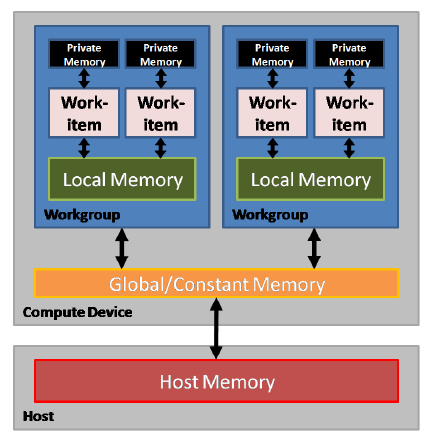
\includegraphics[scale=1]{./graphics/memorymodel.png}
\centering{\caption{Επισκόπιση του μοντέλου μνήμης και οργάνωσης των αντικειμένων εργασίας στο OpenCL.}}
\label{fig7}
\end{figure}

\noindent Η οργάνωση της εσωτερικής μνήμης της GPU στα πλαίσια της εκτέλεσης ενός πυρήνα επεξεργασίας παίζει σημαντικότατο ρόλο στον καθορισμό των επιδόσεών του. Όπως αναφέρθηκε στο κεφάλαιο \ref{chapter:gpgpu}, η αρχιτεκτονική των σύγχρονων GPU δίνει προτεραιότητα  στα υπολογιστικά στοιχεία σε βάρος των στοιχείων μνήμης ή ελέγχου. Ως αποτέλεσμα οι GPU δεν περιέχουν τις πολυεπίπεδες ιεραρχίες κρυφών μνημών που συνηθίζονται στις CPU. Αυτό σημαίνει ότι η πρόσβαση στην γενική μνήμη έχει μεγαλύτερο χρονικό κόστος σε σχέση με τις GPU και, ακόμα σημαντικότερα, ότι ο λόγος του κόστους εντολών μνήμης διά το κόστος εντολών υπολογισμού είναι υψηλότερος στις GPU. Πρακτικά αυτό σημαίνει πως η υπερβολική χρήση της γενικής μνήμης μπορεί να μειώσει σημαντικά την ταχύτητα εκτέλεσης ενός πυρήνα υπολογισμού. Γενικά συνιστάται \cite{AMDIntro} η χρήση της ιδιωτικής ή τοπικής μνήμης αντί της γενικής όπου αυτό είναι εφικτό. Στους πυρήνες υπολογισμού που δημιουργήθηκαν στα πλαίσια αυτής της εργασίας χρησιμοποιούνται αποκλειστικά 
οι καταχωρητές και η ιδιωτική μνήμη του κάθε αντικειμένου εργασίας, καθώς η χωρητικότητα που παρέχουν επαρκεί για την αποθήκευση όλων των δεδομένων που απαιτούνται κατά την εκτέλεση των αλγορίθμων. Επίσης, καθώς δεν υπάρχει ανάγκη μεταφοράς δεδομένων μεταξύ των αντικειμένων εργασίας, δεν χρειάζεται η χρήση τοπικής μνήμης. Η γενική μνήμη χρησιμοποιείται μόνο για την είσοδο και έξοδο δεδομένων προς το σύστημα host.  

Εκτός από την οργάνωση της εσωτερικής μνήμης των GPU, το μοντέλο μνήμης του OpenCL ορίζει και την διαμόρφωση περιοχών μνήμης στο host σύστημα για την είσοδο και έξοδο δεδομένων από και προς την GPU. Στις περισσότερες περιπτώσεις η GPU δεν έχει άμεση πρόσβαση στην κύρια μνήμη του συστήματος host. Τα κοινόχρηστα δεδομένα πρέπει να αντιγραφούν στην μνήμη της GPU μέσω κάποιου διαύλου επικοινωνίας. Στις σύγχρονες GPU ο δίαυλος αυτός είναι σχεδόν πάντα κάποια υλοποίηση του προτύπου PCI Express. Για να βελτιστοποιηθεί η ταχύτητα μεταφοράς των δεδομένων στο δίαυλο αυτό, καθώς και για να διευκολυνθεί η διαδικασία αυτή προγραμματιστικά, το OpenCL χρησιμοποιεί \textit{αντικείμενα ενδιάμεσης μνήμης}. Ένα αντικείμενο ενδιάμεσης μνήμης είναι μια περιοχή μνήμης στο σύστημα host στην οποία αποθηκεύονται δεδομένα με δομή βελτιστοποιημένη για την μεταφορά από και προς την GPU. Υπάρχουν δύο μορφές τέτοιων αντικειμένων: τα αντικείμενα buffer και τα αντικείμενα image. Τα buffer προορίζονται για την αποθήκευση μονοδιάστατων 
δεδομένων. Στα μονοδιάστατα δεδομένα περιλαμβάνονται οι βασικοί τύποι δεδομένων (π.χ. int, float) και οι ορισμένες από τον χρήστη δομές δεδομένων. Ο δεύτερος τύπος αντικειμένων ενδιάμεσης μνήμης, τα image, προορίζονται για την αποθήκευση δι- ή τριδιάστατων δεδομένων όπως εικόνες ή υφές. 

Στην διαδικασία δημιουργίας ενός αντικειμένου μνήμης το OpenCL δίνει την δυνατότητα να προσδιοριστεί ο τρόπος χρήσης του από το σύστημα με την χρήση διαφόρων flag. Οι επιλογές που δίνονται καθορίζουν την πρόσβαση της GPU στο αντικείμενο (αν θα προορίζεται μόνο για ανάγνωση, για εγγραφή ή και τα δύο) τον τρόπο ανάθεσης μνήμης σε αυτό και τον τρόπο μεταφοράς των δεδομένων του στην GPU. Υπάρχουν δύο κύριοι τρόποι ανάθεσης μνήμης. Στον πρώτο, το αντικείμενο ενδιάμεσης μνήμης περιέχει μόνο μια σειρά δεικτών στην περιοχή της κύριας μνήμης που καταλαμβάνει κάποια προϋπάρχουσα δομή δεδομένων (π.χ. πίνακας). Σε αυτή την περίπτωση το αντικείμενο αυτό χρησιμοποιείται απλά ως ενδιάμεσο για την ανάγνωση ή εγγραφή της μνήμης από την GPU. Στον δεύτερο, το εκτελέσιμο του OpenCL αναλαμβάνει την ανάθεση και διαμόρφωση περιοχής στην κύρια μνήμη για την αποθήκευση δεδομένων. Η ανάγνωση και εγγραφή στις περιοχές αυτές γίνεται μόνο μέσω εντολών της διεπαφής προγραμματισμού OpenCL. Η μεταφορά δεδομένων μπορεί να γίνει μέσω άμεσης 
αντιγραφής στην αρχή της εκτέλεσης ή με την τμηματική αντιγραφή των δεδομένων που χρειάζονται όταν αυτά χρησιμοποιούνται για πρώτη φορά από τον πυρήνα υπολογισμού.

Στην υλοποίηση της εργασίας όλα τα αντικείμενα μνήμης είναι τύπου buffer και χρησιμοποιείται ο πρώτος τρόπος ανάθεσης μνήμης. Ο τρόπος μεταφοράς ορίζεται αυτόματα από την εκάστοτε υλοποίηση του OpenCL. Αυτή η επιλογή έγινε καθώς διαπιστώθηκε ότι  προτιμότεροι μέθοδοι μεταφοράς ήταν διαφορετικές ανάμεσα σε GPU διαφορετικών κατασκευαστών. Καθώς οι υλοποιήσεις του OpenCL από κάθε κατασκευαστή GPU στοχεύουν στην μεγιστοποίηση της απόδοσής του στο υλικό που κατασκευάζει ο ίδιος, κρίθηκε προτιμότερο να αφεθεί η επιλογή της ρυθμίσεις αυτών στην υλοποίηση.  

\subsubsection*{Μέθοδος Μεταγλώττισης Πυρήνων}

\noindent Ο διαχωρισμός του κώδικα openCL σε τμήματα που εκτελούνται σε CPU (host πρόγραμμα και τμήματα που εκτελούνται σε GPU (πυρήνες υπολογισμού) έχει ως αποτέλεσμα την χρήση μιας ιδιότυπης μεθόδου μεταγλώττισης. Το host πρόγραμμα μεταγλωττίζεται κανονικά σύμφωνα με τις κοινές μεθόδους της γλώσσας στην οποία είναι γραμμένο (C++ στην περίπτωση της εργασίας αυτής). Ο κώδικας των υπολογιστικών πυρήνων όμως δεν μπορεί να ακολουθήσει αυτή την μέθοδο. Οι πυρήνες στο OpenCL γράφονται σε ένα εξειδικευμένο υποσύνολο της γλώσσας C, την OpenCL C, η οποία βασίζεται στο πρότυπο C99. Ο κώδικας του κάθε πυρήνα είναι (θεωρητικά τουλάχιστον) πλήρως ανεξάρτητος από την συσκευή στην οποία εκτελεστεί. Στην πράξη κάποιες διαφορές στην υλοποίηση του προτύπου OpenCL μεταξύ των διάφορων κατασκευαστών υλικού δημιουργούν την ανάγκη τροποποιήσεων στον κώδικα ανάλογα με την συσκευή για την οποία προορίζεται. Για παράδειγμα, κάποιες γενιές GPU της εταιρίας ATI απαιτούν την χρήση ειδικού κώδικα της εταιρίας αυτής για να μπορέσουν να 
χειριστούν πράξεις κινητής υποδιαστολής διπλής ακρίβειας. 

Οι συμβατές με το OpenCL συσκευές ανήκουν σε πολλές και διαφορετικές αρχιτεκτονικές με θεμελιώδεις διαφορές μεταξύ τους. Η ανίχνευση των συμβατών συσκευών που υπάρχουν σε ένα σύστημα και ο καθορισμός της συσκευής-στόχου γίνεται κατά τον χρόνο εκτέλεσης του προγράμματος host. Όλα αυτά σημαίνουν ότι η μεταγλώττιση των πυρήνων επεξεργασίας πρέπει να γίνεται δυναμικά κατά  την εκτέλεση του προγράμματος host. 
Σχεδόν όλες οι υλοποιήσεις του openCL χρησιμοποιούν για την μεταγλώττιση των πυρήνων επεξεργασίας την υποδομή μεταγλώττισης LLVM (\url{llvm.org}) με εμπρόσθιο τμήμα τον μεταγλωττιστή Clang (\url{clang.llvm.org}). Ο μεταγλωττιστής καλείται κατά την εκτέλεση του προγράμματος host  μέσω κλήσεων που υπάρχουν στο OpenCL API. Το πρόγραμμα host αναλαμβάνει την ανάγνωση του πηγαίου κώδικα του εκάστοτε πυρήνα, τον οποίο τροφοδοτεί στον μεταγλωττιστή με την μορφή συμβολοσειράς. Επίσης, το πρόγραμμα host πρέπει να είναι σε θέση να χειριστεί τα εξαγόμενα του μεταγλωττιστή, είτε αυτά είναι εκτελέσιμο πρόγραμμα, το οποίο πρέπει να μεταφερθεί στην συσκευή-στόχο, είτε είναι μηνύματα λάθους τα οποία πρέπει να παρουσιαστούν στον χρήστη σε κάποια κατάλληλη μορφή.

Στην γενική περίπτωση, αν δεν δοθεί κάποια άλλη οδηγία από τον σχεδιαστή της εφαρμογής, ο κώδικας του κάθε πυρήνα προς εκτέλεση θα μεταγλωττίζεται εκ νέου σε κάθε εκτέλεση του προγράμματος. Για την αποφυγή της άσκοπης καθυστέρησης της εκτέλεσης όταν ένας πυρήνας χρησιμοποιείται επανειλημμένα στο ίδιο σύστημα το OpenCL API παρέχει την δυνατότητα εξαγωγής μιας εκτελέσιμης μορφής ενός μεταγλωττισμένου πυρήνα σε δυαδική μορφή. Η εκτελέσιμη αυτή μορφή μπορεί να αποθηκευθεί σε κάποιο αρχείο, το οποίο μπορεί να χρησιμοποιηθεί άμεσα στις επόμενες εκτελέσεις του προγράμματος παρακάμπτοντας το βήμα της μεταγλώττισης. Το κάθε τέτοιο δυαδικό αρχείο περιέχει μια έτοιμη προς εκτέλεση εκδοχή ενός μόνο πυρήνα για μία μόνο συσκευή.

Στην υλοποίηση της εργασίας η μεταγλώττιση και η παραγωγή των δυαδικών αρχείων έχει αυτοματοποιηθεί. Όταν ζητηθεί η εκτέλεση κάποιου πυρήνα σε κάποια συσκευή το πρόγραμμα host ελέγχει αν υπάρχει στον κατάλογο του προγράμματος αποθηκευμένο δυαδικό αρχείο το οποίο να αντιστοιχεί στο συγκεκριμένο ζεύγος πυρήνα-συσκευής. Αν βρεθεί το ζητούμενο αρχείο τότε το εκτελέσιμο χρησιμοποιείται άμεσα. Αν το αρχείο αυτό δεν βρεθεί τότε καλείται η λειτουργία της μεταγλώττισης και εξάγονται δυαδικά αρχεία για όλες τις συμβατές συσκευές του συστήματος. Τα αρχεία αυτά ονομάζονται ως εξής:
\begin{center}
\verb!Όνομα συσκευής\_Όνομα Πυρήνα.elf!
\end{center}
Το όνομα συσκευής παρατίθεται όπως ακριβώς αναγνωρίζεται από το OpenCL API. H κατάληξη .elf αντιστοιχεί στην παραγόμενη μορφή του εκτελέσιμου \begin{english}(Executable and Linkable Format)\end{english}. 

\subsection{Η βιβλιοθήκη gpuHandler} 
\label{chapter:gpuhandler}
 \noindent Οι λειτουργίες τις οποίες προσφέρει η βιβλιοθήκη \verb!gpuHandler! στα εκτελέσιμα της εργασίας μπορούν να ομαδοποιηθούν ως εξής:

\begin{enumerate}
\item Αναγνώριση της πλατφόρμας εκτέλεσης και εύρεση συσκευών συμβατών με το OpenCL. Εξακρίβωση των δυνατοτήτων των συσκευών αυτών.
\item Μεταγλώττιση του κώδικα του πυρήνα που θα εκτελεστεί στις συσκευές OpenCL ή ανάγνωση ενός ήδη μεταγλωττισμένου πυρήνα. 
\item Διαχείριση των περιοχών ενδιάμεσης μνήμης (buffer) οι οποίες χρησιμοποιούνται για την μεταφορά δεδομένων από και προς την GPU.
\item Εκτέλεση των πυρήνων στην GPU. Είσοδος και έξοδος δεδομένων από την GPU.
\item Βοηθητικές λειτουργίες διαχείρισης λαθών και καθαρισμού της μνήμης.
\end{enumerate}
Αναλυτικότερα, η \verb!gpuHandler! περιέχει τις εξής συναρτήσεις:

\begin{itemize}

\item \textbf{void initializeCL(int deviceNum)}\\ 
H \verb!initializeCL! αρχικοποιεί το περιβάλλον OpenCL στο σύστημα. Η αρχικοποίηση αυτή περιλαμβάνει τρία στάδια: 

\begin{enumerate}
\item Αναγνώριση της πλατφόρμας OpenCL του συστήματος. Πλατφόρμα ονομάζεται η υλοποίηση του OpenCL API από πλευράς software στο εκάστοτε σύστημα. Για παράδειγμα, το AMD APP SDK που χρησιμοποιήθηκε κατά την ανάπτυξη της υλοποίησης αποτελεί μια πλατφόρμα OpenCL. Η αναγνώριση της πλατφόρμας είναι σημαντική επειδή η κάθε πλατφόρμα χρησιμοποιεί μια διαφορετική σειρά εργαλείων για την μεταγλώττιση του κώδικα των πυρήνων και την επικοινωνία με την συσκευή-στόχο. Δεδομένου ότι ο κώδικας της εργασίας προορίζεται κυρίως προς εκτέλεση σε GPU προτιμώνται πλατφόρμες κατασκευασμένες από τις εταιρίες Nvidia ή AMD. Σε περίπτωση που δεν υπάρχουν τέτοιες πλατφόρμες προτιμάται η πρώτη πλατφόρμα που ανιχνεύεται στο σύστημα. 
\item Αναγνώριση και επιλογή της συσκευής-στόχου. Αρχικά λαμβάνεται η λίστα των διαθέσιμων συμβατών συσκευών που αναγνωρίζονται από την πλατφόρμα που επιλέχθηκε. Από αυτές, αν υπάρχει πάνω από μία, επιλέγεται η  συσκευή-στόχος με βάση των αριθμό που δίνεται στο όρισμα deviceNum. Δημιουργείται και αντιστοιχίζεται στη συσκευή-στόχο ένα αντικείμενο τύπου        cl\_command\_queue. Με τα αντικείμενα αυτά το OpenCL αναπαριστά μια σειρά εντολών που αναμένει εκτέλεση σε κάποια συσκευή. Παραδείγματα εντολών που εισέρχονται σε ένα cl\_event είναι η εκτέλεση ενός πυρήνα, η ανάγνωση κάποιου buffer κ.ο.κ.
\item Αναγνώριση του τύπου και του κατασκευαστή της επιλεγμένης συσκευής. Το OpenCL διαχωρίζει τις συσκευές σε τέσσερις γενικές κατηγορίες: CPU, GPU,  επιταχυντές (εξειδικευμένοι επεξεργαστές με μορφή παραπλήσια των GPU αλλά συνήθως χωρίς δυνατότητες επεξεργασίας γραφικών) και λοιπές συσκευές.  Η κατηγορία που ανήκει η συσκευή και το όνομα του κατασκευαστή της χρησιμοποιούνται για τον καθορισμό των τοπικών και γενικών μεγεθών του χώρου προβλήματος όπως αναφέρθηκε στην παράγραφο \ref{chapter:design}. 
\end{enumerate}

\item  \textbf{void allocateInput(int actual\_width, int deviceNum)}\\ 
Η \verb!allocateInput! αναλαμβάνει τον προσδιορισμό του μεγέθους των πινάκων στα οποία αποθηκεύονται τα δεδομένα εισόδου και εξόδου και την ανάθεση θέσεων μνήμης για την αποθήκευσή τους. Οι πίνακες αυτοί περιέχουν το σύνολο των δεδομένων εισόδου και εξόδου που χρησιμοποιούνται σε μια εκτέλεση του προγράμματος και δεν πρέπει να συγχέονται με τις περιοχές ενδιάμεσης μνήμης (buffer), οι οποίες μπορεί να περιέχουν κάποιο υποσύνολό τους ανάλογα με τις συνθήκες εκτέλεσης του προγράμματος. Το μέγεθός τους  ισούται με το αναπροσαρμοσμένο γενικό μέγεθος του χώρου προβλήματος μετά την πρόσθεση εικονικών ζευγών όπως αναφέρεται στην παράγραφο \ref{chapter:design}. Το όρισμα \verb!actual\width! περιέχει τον αριθμό των ζευγών ευθείας-τετραέδρου που διαβάζεται από το αρχείο εισόδου βάσει του οποίου υπολογίζεται το αναπροσαρμοσμένο γενικό μέγεθος. 

Οι θέσεις μνήμης που χρησιμοποιούνται για την αποθήκευση των δεδομένων στους πίνακες είναι ευθυγραμμισμένες σε πολλαπλάσια των 16 Byte, καθώς αυτό απαιτείται από πολλές αρχιτεκτονικές GPU για την σωστή ανάγνωση δεδομένων.

\item \textbf{void allocateBuffers()}\\ 
Η \verb!allocateBuffers! δημιουργεί τα αντικείμενα ενδιάμεσης μνήμης που χρησιμοποιούνται από το πρόγραμμα. Η συνάρτηση προσδιορίζει μόνο τα δικαιώματα πρόσβασης της GPU στα αντικείμενα, δηλαδή την διάκριση μεταξύ αυτών που δέχονται μόνο ανάγνωση από την GPU (δεδομένα εισόδου) και αυτών που δέχονται μόνο εγγραφή (δεδομένα εξόδου). Ο τρόπος ανάθεσης περιοχών μνήμης σε αυτά γίνεται αυτόματα από την υλοποίηση του OpenCL. Επίσης, η συνάρτηση αυτή αναλαμβάνει τον ορισμό των περιοχών ενδιάμεσης μνήμης ως ορίσματα στους πυρήνες επεξεργασίας.

\item \textbf{void runCLKernelsWithIO()}\\ 
Η \verb!runCLKernelsWithIO! περιλαμβάνει την μεταφορά των δεδομένων εισόδου από τους αντίστοιχους πίνακες στις περιοχές ενδιάμεσης μνήμης, την εκκίνηση της εκτέλεσης ενός πυρήνα επεξεργασίας και την ανάκτηση των δεδομένων εξόδου από την GPU. Η μεταφορά των δεδομένων εισόδου γίνεται με κλήση στην συνάρτηση \verb!writeBuffers! και, αντίστοιχα, η ανάκτηση των δεδομένων εξόδου γίνεται με την \verb!readBuffers!. 

Η \verb!runCLKernelsWithIO! μπορεί να διαχωρίσει την επεξεργασία των δεδομένων σε πάνω από μία εκτέλεση του πυρήνα. Ο διαχωρισμός αυτός γίνεται με βάση την χωρητικότητα της μνήμης της GPU στόχου. Σε περίπτωση που χρειαστεί διαχωρισμός υπολογίζεται ο μέγιστος αριθμός εγγραφών (ζευγών ευθείας-τετραέδρου) που μπορεί να χειριστεί η GPU σε μια εκτέλεση. Για να ικανοποιούνται οι περιορισμοί που αναφέρθηκαν στην παράγραφο \ref{chapter:design}, ο αριθμός αυτός περικόπτεται στο αμέσως μικρότερο ακέραιο πολλαπλάσιο του τοπικού μεγέθους. Ο αριθμός αυτός ορίζεται ως νέο ολικό μέγεθος. Κάθε εκτέλεση του πυρήνα γίνεται με το νέο αυτό ολικό μέγεθος, λαμβάνοντας ως στοιχεία εισόδου ένα υποσύνολο των πινάκων εισόδου και παράγοντας την αντίστοιχη έξοδο.

Η εκτέλεση του πυρήνα στην GPU, όπως και όλες οι εντολές που απευθύνονται στην συσκευή-στόχο στο OpenCL, προστίθεται στην σειρά εντολών της συσκευής. Η σειρά εντολών, η οποία εκτελείται στην GPU, λειτουργεί ασύγχρονα με το host πρόγραμμα το οποίο εκτελείται στην CPU. Για να είναι δυνατόν το host πρόγραμμα να γνωρίζει ότι η εκτέλεση ενός πυρήνα έχει τερματιστεί χρησιμοποιούνται αντικείμενα της κλάσης \verb!cl_event!. Τα \verb!cl_event! αποτελούν την μέθοδο συγχρονισμού μεταξύ του host προγράμματος και της GPU. Κάθε αντικείμενο της κλάσης \verb!cl_event! αντιστοιχεί σε μία εντολή στην σειρά εντολών. Για τις περιπτώσεις που είναι προγραμματιστικά αναγκαίο το host πρόγραμμα να αναμείνει κάποια διαδικασία στην GPU το OpenCL παρέχει συναρτήσεις οι οποίες αναστέλλουν την λειτουργία του host προγράμματος μέχρι το αντίστοιχο \verb!cl_event! να χαρακτηριστεί ολοκληρωμένο. Ο μηχανισμός αυτός χρησιμοποιείται στο host πρόγραμμα της εργασίας για να αναστείλει την εκτέλεσή του εν αναμονή της ολοκλήρωσης της επεξεργασίας 
του πυρήνα.  


\item \textbf{void runCLKernels()}\\ 
Η \verb!runCLKernels! περιέχει μόνο το τμήμα της εκτέλεσης του πυρήνα της \verb!runCLKernelsWithIO!, χωρίς τον κώδικα διαχωρισμού και τις κλήσεις εισόδου-εξόδου. Χρησιμοποιείται αποκλειστικά από το εκτελέσιμο Bench για την μέτρηση του καθαρού χρόνου επεξεργασίας στην GPU, ξεχωρίζοντας τον από τον χρόνο που απαιτείται για την ανάγνωση και εγγραφή των περιοχών ενδιάμεσης μνήμης. Αυτό επιτρέπει την ξεχωριστή χρονομέτρηση των χρόνων ανάγνωσης, εγγραφής και εκτέλεσης, δίνοντας περισσότερες πληροφορίες για την απόδοση της υλοποίησης σε GPU.


\item \textbf{void writeBuffers(cl\_uint offset, cl\_uint entriesToWrite)}\\ 
H \begin{english}\verb!writeBuffers!\end{english} μεταφέρει έναν αριθμό εγγραφών ίσο με το όρισμα \begin{english}\verb!entriesToWrite!\end{english} από τους πίνακες εισόδου στις περιοχές ενδιάμεσης μνήμης. Η ανάγνωση των πινάκων αρχίζει από την θέση offset. Αυτό επιτρέπει την μεταφορά ενός υποσυνόλου των δεδομένων των πινάκων εισόδου αν αυτό χρειαστεί. 


\item \textbf{void readBuffers(cl\_uint offset, cl\_uint entriesToRead)}\\ 
Αντίστοιχα με την \begin{english}\verb!writeBuffers!\end{english}, η \begin{english}\verb!readBuffers!\end{english} μεταφέρει \begin{english}\verb!entriesToRead!\end{english} εγγραφές από τις περιοχές ενδιάμεσης μνήμης στους πίνακες εξόδου, αρχίζοντας από την θέση offset.



\item \textbf{void makeCLKernel(const char *kernelName, int deviceNum)}\\ 
Η \verb!makeCLKernel! αναλαμβάνει την δημιουργία του πυρήνα υπολογισμού που θα εκτελεστεί στην GPU. Ο πυρήνας μπορεί να είναι ήδη μεταγλωττισμένος και αποθηκευμένος σε δυαδικό αρχείο ή να βρίσκεται σε μορφή πηγαίου κώδικα. Αρχικά, η \verb!makeCLKernel! προσδιορίζει το όνομα του δυαδικού αρχείου το οποίο αντιστοιχεί στον συνδυασμό πυρήνα-συσκευής που χρησιμοποιείται. Το όνομα του πυρήνα καθορίζεται από τις παραμέτρους που δίδονται στο πρόγραμμα από τον χρήστη και περιέχεται στο όρισμα \verb!kernelName!. Το όνομα της συσκευής αναγνωρίζεται από το OpenCL με βάση τον αριθμό \verb!deviceNum!. Τα δυαδικά αρχεία  ονομάζονται σύμφωνα με τον κανόνα που παρουσιάστηκε στην παράγραφο \ref{chapter:design}. Αν βρεθεί δυαδικό αρχείο με το προβλεπόμενο όνομα στον φάκελο του προγράμματος τότε το αρχείο αυτό διαβάζεται και χρησιμοποιείται για την δημιουργία του πυρήνα. Αλλιώς, αν δεν βρεθεί το ζητούμενο αρχείο, αρχίζει η διαδικασία της μεταγλώττισης από τον πηγαίο κώδικα. Το αρχείο κειμένου που περιέχει τον πηγαίο κώδικα του 
ζητούμενο πυρήνα διαβάζεται και μετατρέπεται σε συμβολοσειρά μέσω της συνάρτησης \verb!convertToString!. Η συμβολοσειρά αυτή τροφοδοτείται στον ενσωματωμένο μεταγλωττιστή της υλοποίησης του OpenCL. Η μεταγλώττιση γίνεται ξεχωριστά για όλες τις συμβατές με το OpenCL συσκευές που υπάρχουν στο σύστημα. Αν κατά την μεταγλώττιση του πυρήνα παρουσιαστεί κάποιο λάθος τότε τα μηνύματα λάθους που εξάγονται από τον μεταγλωττιστή παρουσιάζονται στον χρήστη και η εκτέλεση διακόπτεται. Αν η μεταγλώττιση είναι επιτυχής η δυαδική μορφή του πυρήνα που παράγεται αποθηκεύεται σε δυαδικό αρχείο μέσω της συνάρτησης \verb!dumpBinary! και χρησιμοποιείται στο υπόλοιπο του προγράμματος.


\item \textbf{void dumpBinary(cl\_program program, const char *kernelName)}\\ 
Η dumpBinary χρησιμοποιείται για την εξαγωγή ενός επιτυχώς μεταγλωττισμένου πυρήνα από την \verb!makeCLKernel! σε μορφή δυαδικού αρχείου. Καθώς η μεταγλώττιση της \verb!makeCLKernel! γίνεται για όλες τις συμβατές συσκευές που υπάρχουν στο σύστημα, η \verb!dumpbinary! εξάγει ένα δυαδικό αρχείο ανά συσκευή.

\item \textbf{std::string convertToString(const char *filename)}\\ 
Η \verb!convertToString! μετατρέπει τα περιεχόμενα ενός αρχείου κειμένου σε μια συμβολοσειρά τύπου \verb!std::string!. Χρησιμοποιείται για την μετατροπή των αρχείων κειμένου που περιέχουν πηγαίο κώδικα πυρήνων σε μορφή κατάλληλη για είσοδο στον μεταγλωττιστή του OpenCL.


\item \textbf{void cleanupCL()}\\ 
Η \verb!cleanupCL! καλείται κατά τον τερματισμό του προγράμματος. Χρησιμοποιείται για την διαγραφή και την απελευθέρωση της μνήμης όλων των αντικειμένων του προγράμματος που έχουν σχέση με το OpenCL. Παραδείγματα τέτοιων αντικειμένων είναι οι μεταγλωττισμένοι πυρήνες \verb!cl_program!, οι σειρές εντολών \verb!cl_command_queue!, τα \verb!cl_event! κ.τ.λ. 


\item \textbf{void cleanupHost()}\\ 
H \verb!cleanupHost! καλείται κατά τον τερματισμό του προγράμματος και χρησιμοποιείται για την διαγραφή και την απελευθέρωση της μνήμης των πινάκων εισόδου-εξόδου δεδομένων.


\item \textbf{void exitOnError(const char *error\_text)}\\ 
Η \verb!exitOnError! καλείται αν εμφανιστεί κάποιο λάθος κατά τον χρόνο εκτέλεσης του προγράμματος. Εκτυπώνει το κατάλληλο μήνυμα λάθους και τερματίζει το πρόγραμμα. Αν το λάθος εμφανιστεί σε κάποια κλήση του OpenCL API εκτυπώνεται και ο κωδικός λάθους όπως ορίζεται από το πρότυπο του OpenCL.  

\end{itemize}

\subsection{Πυρήνες υπολογισμού} 

\noindent Οι πυρήνες υπολογισμού αναπτύχθηκαν με προσαρμογή του ακολουθιακού κώδικα στις σχεδιαστικές επιλογές που επιβάλλονται από την OpenCL C. Δημιουργήθηκαν οι εξής τέσσερις πυρήνες:
\begin{itemize*}
\item RayTetraSegura0.cl: Βασικός αλγόριθμος (μορφή 0) συντεταγμένων Plücker.
\item RayTetraSTP0.cl: Βασικός αλγόριθμος (μορφή 0) μεικτού γινόμενου.
\item RayTetraSTP1.cl: Αλγόριθμος μεικτού γινόμενου με βελτιστοποιήσεις ελέγχου και επανάληψη χρήσης υπολογισμένων ποσοτήτων (μορφή 1).
\item RayTetraSTP2.cl: Αλγόριθμος μεικτού γινόμενου με βελτιστοποιήσεις ελέγχου, επανάληψη χρήσης υπολογισμένων ποσοτήτων και γεωμετρική βελτιστοποίηση (μορφή 2).
\end{itemize*}
Ο κώδικας των πυρήνων ακολουθεί σε μεγάλο βαθμό την μορφή της ακολουθιακής. Μεταξύ των δύο μορφών εμφανίζονται δύο βασικές διαφορές: 

Πρώτον, η διανυσματοποίηση των δεδομένων. H OpenCL C παρέχει ειδικούς τύπους δεδομένων που προορίζονται για την αναπαράσταση διανυσμάτων. Οι τύποι αυτοί είναι επεκτάσεις των βασικών αριθμητικών τύπων της C (float,double κ.τ.λ.) οι οποίες ονομάζονται με βάση των αριθμό των συνισταμένων που περιέχουν ή, αντίστοιχα, με τον αριθμό των διαστάσεων του διανυσματικού χώρου στον οποίο αντιστοιχούν. Για παράδειγμα, ένα διδιάστατο διάνυσμα με συνισταμένες αριθμούς κινητής υποδιαστολής μονής ακρίβειας ονομάζεται float2, ενώ ένα τετραδιάστατο με αριθμούς διπλής ακρίβειας double4. 

Η χρήση διανυσματικών δεδομένων έχει μεγάλη σημασία για την απόδοση των πυρήνων σε κάποιες αρχιτεκτονικές GPU (ιδιαίτερα σε αυτές της AMD). Η αρχιτεκτονική των σύγχρονων GPU περιέχει πολύ αποτελεσματικές μεθόδους επεξεργασίας διανυσματικών υπολογισμών καθώς σε αυτούς στηρίζεται μεγάλο μέρος της επεξεργασίας γραφικών. Το γεγονός αυτό επιδεικνύεται από το εκτενές σύνολο βελτιστοποιημένων διανυσματικών εντολών που υπάρχει στο πρότυπο του OpenCL \cite{OpenCLSpec}. Ανάμεσα στις εντολές αυτές υπάρχουν υλοποιήσεις του εσωτερικού (dot) και εξωτερικού (cross) γινομένου οι οποίες υλοποιούν το μεγαλύτερο μέρος των διανυσματικών υπολογισμών που είναι απαραίτητοι για τους αλγόριθμους της εργασίας.

Στον κώδικα των πυρήνων όλα τα δεδομένα των αλγορίθμων τα οποία αντιστοιχούν σε διανύσματα αποθηκεύονται σε διανυσματικούς τύπους του OpenCL. Αν και όλα τα διανύσματα που χρησιμοποιούνται είναι τριδιάστατα,  για την αναπαράστασή τους χρησιμοποιείται ο τύπος double4. Η τέταρτη συνισταμένη των διανυσμάτων αυτών παίρνει την τιμή 0. Αυτό γίνεται επειδή πολλές GPU υποστηρίζουν μόνο διανύσματα με αριθμό συνισταμένων ίσο με δύναμη του 2 (συνήθως 2,4,8 ή 16). 

Δεύτερον, η προσθήκη βοηθητικού κώδικα για την παράλληλη εκτέλεση. Ο βοηθητικός κώδικας για την παράλληλη εκτέλεση έχει ως σκοπό την εύρεση του αριθμού του αντικειμένου εργασίας στο οποίο εκτελείται. Με βάση τον αριθμό αυτό υπολογίζονται οι θέσεις των δεδομένων εισόδου των ενδιάμεσων περιοχών μνήμης και εξόδου που αντιστοιχούν στο συγκεκριμένο αντικείμενο εργασίας.

\section{Χρήση Προγράμματος}

\subsection{Απαιτήσεις υλικού και λογισμικού}
\noindent Η υλοποίηση σε OpenCL προορίζεται κυρίως προς εκτέλεση σε GPU των εταιριών AMD και Nvidia. Ειδικότερα οι GPU της Nvidia πρέπει να υποστηρίζουν τουλάχιστον το CUDA Compute Capability 1.3 καθώς αυτό απαιτείται για την εκτέλεση υπολογισμών με αριθμούς διπλής ακρίβειας.  Επιπλέον υποστηρίζονται και CPU κατασκευασμένες από την AMD συμβατές με το σύνολο εντολών SSE2 ή από την Intel συμβατές με το SSE4. Η λίστα των  συμβατών συσκευών με το OpenCL διατηρείται από το Khronos Group στην διεύθυνση \url{http://www.khronos.org/conformance/adopters/conformant-products/}.

Από την πλευρά του λογισμικού απαιτείται η εγκατάσταση ενός περιβάλλοντος προγραμματισμού ΟpenCL συμβατού με την  συσκευή στην οποία θα εκτελεστεί η εφαρμογή. Για τις CPU και GPU της AMD αυτό είναι το AMD APP SDK (\url{http://developer.amd.com/sdks/amdappsdk/downloads/pages/default.aspx} ), για τις CPU της Intel το Intel OpenCL SDK  (\url{http://software.intel.com/en-us/articles/opencl-sdk/}) και για τις GPU της Nvidia το Nvidia CUDA Toolkit  (\url{http://developer.nvidia.com/cuda-toolkit}). 
 
\subsection{Μεταγλώττιση}
\noindent Ο κώδικας της εργασίας έχει διαμορφωθεί σε δύο εκδόσεις. Η μία από αυτές προορίζεται για χρήση σε λειτουργικό σύστημα Linux. Η μεταγλώττισή της γίνεται μέσω makefile το οποίο βρίσκεται στον φάκελο \verb!RayTetra! και προορίζεται για χρήση με τον μεταγλωττιστή \verb!g++!. Η έκδοση αυτή απαιτεί, πέρα από όσα αναφέρθηκαν στην προηγούμενη παράγραφο, να είναι εγκατεστημένη στο σύστημα κάποια υλοποίηση της βιβλιοθήκης \verb!glut! (\begin{english}OpenGL Utility Toolkit\end{english}). 

Η δεύτερη έκδοση προορίζεται για τα λειτουργικά συστήματα της οικογένειας Windows. Η έκδοση αυτή είναι στην μορφή ενός Solution για το περιβάλλον ανάπτυξης \begin{english}Visual Studio\end{english} 2008. Καθένα από τα εκτελέσιμα \verb!RayTetra!, \verb!RandomRayTetra! και \verb!Bench! δημιουργείται από ένα ξεχωριστό ομώνυμο \begin{english}Project\end{english} μέσα στο \begin{english}Solution\end{english} αυτό. Η έκδοση αυτή περιλαμβάνει την βιβλιοθήκη \begin{english}GLUT for Win32\end{english} του \begin{english}Nate Robins\end{english} (\url{http://user.xmission.com/~nate/glut.html}) και την υλοποίηση σε περιβάλλον Windows της βιβλιοθήκης \verb!getopt! από τον \begin{english}Ludvik Jerabek\end{english} (\url{http://www.codeproject.com/KB/cpp/getopt4win.aspx}), η οποία χρησιμοποιείται στον κώδικα για την ευκολότερη επεξεργασία των ορισμάτων γραμμής εντολών κατά την κλήση των εκτελέσιμων.

\subsection{Χρήση} 
\noindent Από τα εκτελέσιμα που αναφέρθηκαν στην παράγραφο \ref{chapter:initial} η χρήση GPU και ο ακολουθιακός αλγόριθμος μεικτού γινομένου έχουν ενσωματωθεί στα εκτελέσιμα \verb!RayTetra! και \verb!Bench!. Επίσης, έχουν προστεθεί δύο βοηθητικά bash script, τα \verb!result\_compare.sh! και \verb!fullbench.sh!, τα οποία έχουν ως σκοπό την επαλήθευση των αποτελεσμάτων του \verb!RayTetra! και την διευκόλυνση της μέτρησης των επιδόσεων με το \verb!Bench! αντίστοιχα. Για την οπτικοποίηση των αποτελεσμάτων των που παράγονται από το \begin{english}\verb!fullbench.sh!\end{english} έχει προστεθεί ένα bash script, το \begin{english}\verb!plot\_time\_graph.sh!\end{english},το οποίο παράγει διαγράμματα επιδόσεων με βάση τα εξαγόμενα του \begin{english}\verb!fullbench.sh!\end{english}. Η δημιουργία των διαγραμμάτων γίνεται μέσω του εργαλείου \verb!gnuplot! (\url{http://www.gnuplot.info}). Η μορφή των διαγραμμάτων εξηγείται στο κεφάλαιο \ref{chapter:bench_method}. 

Όλα τα bash script που αναφέρθηκαν είναι διαθέσιμα μόνο στην έκδοση  που προορίζεται για χρήση σε Linux, καθώς η λειτουργία τους εξαρτάται από εργαλεία που είναι διαθέσιμα μόνο σε αυτό το περιβάλλον.

\noindent Τα εκτελέσιμα χρησιμοποιούνται ως εξής:\\ 

\noindent\textbf{\verb!RayTetra!}\\
Σύνταξη: 
./RayTetra [αλγόριθμος] [επιλογές] [αρχείο εισόδου] 
[αρχείο εξόδου] [αριθμός επαναλήψεων]

\noindent Οι επιλογές αλγορίθμων που είναι σχετικές με την εργασία είναι:
\begin{itemize}
\item -t i: Ακολουθιακός αλγόριθμος μεικτού γινομένου μορφής i, όπου i=0,1,2.
\item -g i: Υλοποίηση σε OpenCL αλγορίθμου i, όπου i=0,1,2,3 
	\\0=Βασικός Αλγόριθμος συντεταγμένων Plücker(μορφή 0)
	\\1=Βασικός Αλγόριθμος μεικτού γινόμενου(μορφή 0)
	\\2=Αλγόριθμος μεικτού γινόμενου(μορφή 1)
	\\3=Αλγόριθμος μεικτού γινόμενου(μορφή 2)
\end{itemize}

\noindent Οι πιθανές επιλογές είναι:
\begin{itemize}
\item -h:   Εκτύπωση μηνύματος βοήθειας και έξοδος.\\
\item -p i: Επιλογή του τι θα εκτυπωθεί στο αρχείο εξόδου:\\
      i=t: Εκτύπωση χρόνου\\
      i=r: Εκτύπωση αποτελεσμάτων\\
      i=b: Εκτύπωση και των δύο (προεπιλεγμένο)\\
\item -d i: Υπολογισμός και εμφάνιση με γραφικά της γραμμής i του αρχείου εισόδου. Αν χρησιμοποιηθεί τότε τα ορίσματα [αρχείο εξόδου] [αριθμός επαναλήψεων] αγνοούνται.
\item -n i: Χρήση της συσκευής OpenCL με αριθμό i για τους αλγορίθμους OpenCL. Παρέχεται για τα συστήματα με πάνω από μία συμβατή συσκευή. Το i είναι θετικός ακέραιος $\geq$ 0. Η προεπιλεγμένη τιμή είναι 0, δηλαδή η πρώτη συμβατή συσκευή που βρίσκεται στο σύστημα.\\
\end{itemize}

\noindent\textbf{\verb!Bench!}\\
Σύνταξη:  ./Bench [αρχείο εισόδου] [αρχείο εξόδου] [αριθμός επαναλήψεων] [αριθμός συσκευής OpenCL]

\noindent Το προαιρετικό όρισμα [αριθμός συσκευής OpenCL] χρησιμοποιείται ακριβώς όπως και η τιμή της επιλογής -n του \verb!RayTetra!.\\
           
\noindent\textbf{\verb!RandomRayTetra!}\\
Σύνταξη:  ./RandomRayTetra [αρχείο εξόδου] -i [αριθμός τεμνόμενων ζευγών] -n [αριθμός μη τεμνόμενων ζευγών]\\

\noindent Τα bash script χρησιμοποιούνται ως εξής: \\

\noindent\textbf{\verb!result\_compare.sh!}\\
Σύνταξη:\\
\begin{itemize}
\item Μέθοδος 1: Δημιουργία νέου αρχείου εισόδου μέσω του \verb!RayTetra!.\\
./result\_compare [αριθμός τεμνόμενων ζευγών] [αριθμός μη τεμνόμενων ζευγών] [όνομα για το νέο αρχείο εισόδου] [αριθμός συσκευής OpenCL]
\item Μέθοδος 2: Χρήση υπάρχοντος αρχείου εισόδου.\\
 ./result\_compare [αρχείο εισόδου]  [αριθμός συσκευής OpenCL]   
\end{itemize} 
\noindent Εκτελεί ελέγχους τομής μέσω του \verb!RayTetra! για τον αριθμό ζευγών που δίνεται ως όρισμα. Χρησιμοποιεί το ίδιο αρχείο εισόδου σε όλες τις υλοποιήσεις όλων των αλγορίθμων και συγκρίνει τα αποτελέσματα για πιθανές διαφορές. Η σύγκριση γίνεται μέσω του προγράμματος \verb!diff! του πακέτου GNU Diffutils σε περιβάλλον Linux. Τα αποτελέσματα της σύγκρισης εκτυπώνονται σε αρχείο που παίρνει το όνομα [αρχείο εισόδου].differences.\\

\noindent\textbf{\verb!fullbench.sh!}\\
Σύνταξη: ./fullbench.sh [αριθμός ζευγών] [αριθμός επαναλήψεων] [βήμα ποσοστού τεμνόμενων ζευγών] [αριθμός συσκευής OpenCL] 
 
\noindent Μετρά τον χρόνο εκτέλεσης των αλγορίθμων για έναν δοσμένο αριθμό ζευγών. Στον πρώτο έλεγχο όλα τα ζεύγη είναι μη τεμνόμενα. Σε κάθε επόμενο το ποσοστό τοις εκατό των τεμνόμενων ζευγών αυξάνεται σύμφωνα με το [βήμα ποσοστού τεμνόμενων ζευγών]. Για παράδειγμα, αν το βήμα είχε τιμή 20 θα γίνονταν 6 έλεγχοι με ποσοστά 0\%, 20\%, 40\%, 60\%, 80\% και 100\% κατά σειρά. Η κάθε μέτρηση γίνεται σε όσες επαναλήψεις οριστούν από το [αριθμός επαναλήψεων]. Τα αποτελέσματα αποθηκεύονται σε μορφή CSV στο αρχείο output.csv στον φάκελο \verb!RayTetra!. Οι στήλες του CSV διαχωρίζονται με τον χαρακτήρα του κόμματος και οι γραμμές με τον χαρακτήρα αλλαγής γραμμής. Επίσης, το \verb!fullbench.sh! περιέχει κλήσεις προς το \begin{english}\verb!plot\_time\_graph.sh!\end{english} για την παραγωγή διαγραμμάτων με βάση τα αποτελέσματά του.   


\UndefineShortVerb{\!}




